\chapter{Architectural and workflow design patterns}

\section{Engineering principles}

Workflow patterns describe coordination and control, not a particular vendor implementation. A workflow with predetermined stages is not necessarily an autonomous agent; an agent may be invoked inside one stage. The pattern catalog distinguishes selection, decomposition, review, verification, state and approval. Compose patterns only where their additional complexity pays for itself.

\section{Implementation approach}

Use the catalog to choose a minimal architecture: specification-driven work plus generator-verifier is a good baseline for a bounded feature. Add an independent reviewer when defect impact is high. Add orchestration only when tasks can be decomposed and integrated without shared mutable state. Keep each state transition explicit.

\section{Verification and limitations}

Each pattern below specifies applicability, execution structure, trade-offs and an external implementation approach usable with either adapter. No entry claims a native feature unless identified separately in the platform chapters.

Figure~\ref{fig:d11} illustrates the conceptual flow from Inspect to Implement. The edges describe the proposed integration or control relationship, not undocumented internal calls.

\begin{figure}[htbp]\centering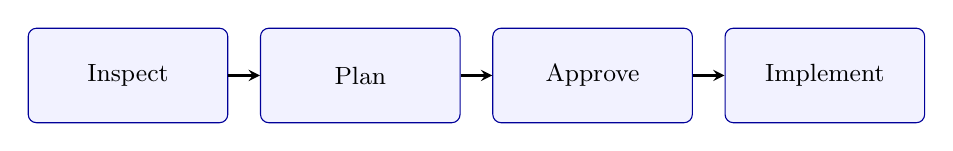
\begin{tikzpicture}[nodebox/.style={draw=blue!60!black,fill=blue!5,rounded corners=3pt,minimum height=12mm,text width=23mm,align=center,font=\small},>=stealth]
\node[nodebox] (n0) at (0.00,0.00) {Inspect};
\node[nodebox] (n1) at (2.95,0.00) {Plan};
\node[nodebox] (n2) at (5.90,0.00) {Approve};
\node[nodebox] (n3) at (8.85,0.00) {Implement};
\draw[->,thick] (n0.east) -- (n1.west);
\draw[->,thick] (n1.east) -- (n2.west);
\draw[->,thick] (n2.east) -- (n3.west);
\end{tikzpicture}
\caption{Plan and execute (conceptual view).}\label{fig:d11}\end{figure}

Figure~\ref{fig:d12} illustrates the conceptual flow from Coordinator to Integrate. The edges describe the proposed integration or control relationship, not undocumented internal calls.

\begin{figure}[htbp]\centering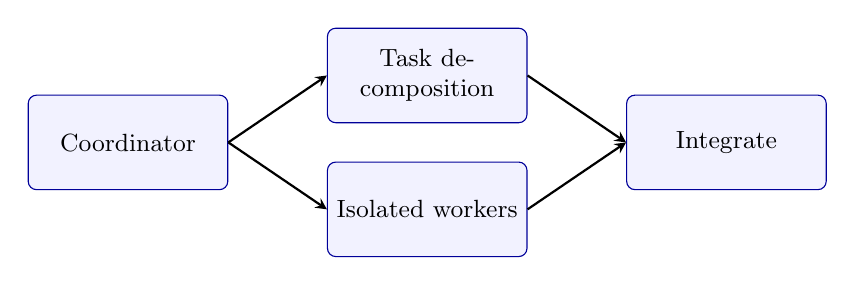
\begin{tikzpicture}[nodebox/.style={draw=blue!60!black,fill=blue!5,rounded corners=3pt,minimum height=12mm,text width=23mm,align=center,font=\small},>=stealth]
\node[nodebox] (n0) at (0.00,0.00) {Coordinator};
\node[nodebox] (n1) at (3.80,0.85) {Task decomposition};
\node[nodebox] (n2) at (3.80,-0.85) {Isolated workers};
\node[nodebox] (n3) at (7.60,0.00) {Integrate};
\draw[->,thick] (n0.east) -- (n1.west);
\draw[->,thick] (n0.east) -- (n2.west);
\draw[->,thick] (n1.east) -- (n3.west);
\draw[->,thick] (n2.east) -- (n3.west);
\end{tikzpicture}
\caption{Orchestrator and worker (conceptual view).}\label{fig:d12}\end{figure}

Figure~\ref{fig:d13} illustrates the conceptual flow from Writer to Decision. The edges describe the proposed integration or control relationship, not undocumented internal calls.

\begin{figure}[htbp]\centering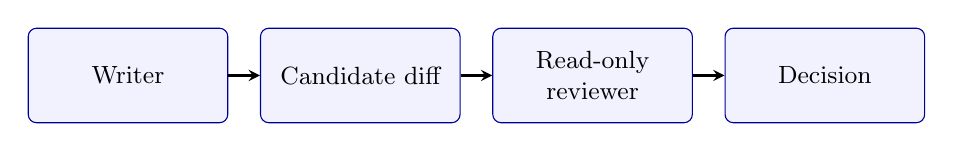
\begin{tikzpicture}[nodebox/.style={draw=blue!60!black,fill=blue!5,rounded corners=3pt,minimum height=12mm,text width=23mm,align=center,font=\small},>=stealth]
\node[nodebox] (n0) at (0.00,0.00) {Writer};
\node[nodebox] (n1) at (2.95,0.00) {Candidate diff};
\node[nodebox] (n2) at (5.90,0.00) {Read-only reviewer};
\node[nodebox] (n3) at (8.85,0.00) {Decision};
\draw[->,thick] (n0.east) -- (n1.west);
\draw[->,thick] (n1.east) -- (n2.west);
\draw[->,thick] (n2.east) -- (n3.west);
\end{tikzpicture}
\caption{Implementer and reviewer (conceptual view).}\label{fig:d13}\end{figure}

Figure~\ref{fig:d14} illustrates the conceptual flow from Generator to Pass or repair. The edges describe the proposed integration or control relationship, not undocumented internal calls.

\begin{figure}[htbp]\centering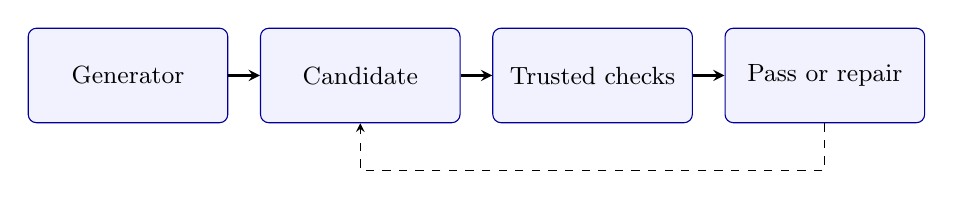
\begin{tikzpicture}[nodebox/.style={draw=blue!60!black,fill=blue!5,rounded corners=3pt,minimum height=12mm,text width=23mm,align=center,font=\small},>=stealth]
\node[nodebox] (n0) at (0.00,0.00) {Generator};
\node[nodebox] (n1) at (2.95,0.00) {Candidate};
\node[nodebox] (n2) at (5.90,0.00) {Trusted checks};
\node[nodebox] (n3) at (8.85,0.00) {Pass or repair};
\draw[->,thick] (n0.east) -- (n1.west);
\draw[->,thick] (n1.east) -- (n2.west);
\draw[->,thick] (n2.east) -- (n3.west);
\draw[->,dashed] (n3.south) -- ++(0,-.6) -| (n1.south);
\end{tikzpicture}
\caption{Generator and verifier (conceptual view).}\label{fig:d14}\end{figure}

\subsection{Interactive steering}

\textbf{Applicability and intent.} Ambiguous design. \textbf{Roles.} Engineer; agent.

\textbf{Execution.} Question > propose > discuss > revise. \textbf{Trade-off.} Fast clarification; human attention required.

\textbf{Failure and control.} Agent assumes approval; require explicit decision. \textbf{Example.} Resolve a public API ambiguity.

Both platforms: apply the sequence externally using a reviewed adapter; native feature equivalence is not assumed.

\begin{center}\small \textsf{Question} $\rightarrow$ \textsf{propose} $\rightarrow$ \textsf{discuss} $\rightarrow$ \textsf{revise}\end{center}

\subsection{Autonomous task delegation}

\textbf{Applicability and intent.} Bounded reversible change. \textbf{Roles.} Sponsor; worker; verifier.

\textbf{Execution.} Contract > execute > verify > report. \textbf{Trade-off.} Low coordination; weak specifications cause drift.

\textbf{Failure and control.} Scope expansion; enforce workspace policy. \textbf{Example.} Fix a failing unit test.

Both platforms: apply the sequence externally using a reviewed adapter; native feature equivalence is not assumed.

\begin{center}\small \textsf{Contract} $\rightarrow$ \textsf{execute} $\rightarrow$ \textsf{verify} $\rightarrow$ \textsf{report}\end{center}

\subsection{Plan-and-execute}

\textbf{Applicability and intent.} Multi-step change. \textbf{Roles.} Planner; executor; reviewer.

\textbf{Execution.} Inspect > plan > approve > execute. \textbf{Trade-off.} Early risk discovery; plan can become stale.

\textbf{Failure and control.} Revalidate baseline before execution. \textbf{Example.} Upgrade an API client.

Both platforms: apply the sequence externally using a reviewed adapter; native feature equivalence is not assumed.

\begin{center}\small \textsf{Inspect} $\rightarrow$ \textsf{plan} $\rightarrow$ \textsf{approve} $\rightarrow$ \textsf{execute}\end{center}

\subsection{Specification-driven development}

\textbf{Applicability and intent.} Clear desired behavior. \textbf{Roles.} Spec owner; worker; test runner.

\textbf{Execution.} Spec > acceptance tests > patch > gate. \textbf{Trade-off.} Traceability; specification effort.

\textbf{Failure and control.} Test tampering; protect acceptance tests. \textbf{Example.} Discount calculator.

Both platforms: apply the sequence externally using a reviewed adapter; native feature equivalence is not assumed.

\begin{center}\small \textsf{Spec} $\rightarrow$ \textsf{acceptance tests} $\rightarrow$ \textsf{patch} $\rightarrow$ \textsf{gate}\end{center}

\subsection{Test-driven agentic development}

\textbf{Applicability and intent.} Behavior can be isolated. \textbf{Roles.} Test author; implementer; verifier.

\textbf{Execution.} Red test > minimal patch > green test > refactor. \textbf{Trade-off.} Fast feedback; narrow tests miss defects.

\textbf{Failure and control.} False green; run independent suite. \textbf{Example.} Boundary validation.

Both platforms: apply the sequence externally using a reviewed adapter; native feature equivalence is not assumed.

\begin{center}\small \textsf{Red test} $\rightarrow$ \textsf{minimal patch} $\rightarrow$ \textsf{green test} $\rightarrow$ \textsf{refactor}\end{center}

\subsection{Prompt chaining}

\textbf{Applicability and intent.} Known sequence of transformations. \textbf{Roles.} Stage controller; agent.

\textbf{Execution.} Extract > transform > validate. \textbf{Trade-off.} Simple composition; propagation of error.

\textbf{Failure and control.} Validate intermediate schema. \textbf{Example.} Turn issue into test cases.

Both platforms: apply the sequence externally using a reviewed adapter; native feature equivalence is not assumed.

\begin{center}\small \textsf{Extract} $\rightarrow$ \textsf{transform} $\rightarrow$ \textsf{validate}\end{center}

\subsection{Sequential workflows}

\textbf{Applicability and intent.} Dependent tasks. \textbf{Roles.} Controller; stage workers.

\textbf{Execution.} Analyze > implement > test > review. \textbf{Trade-off.} Predictable ordering; limited concurrency.

\textbf{Failure and control.} Halt on failed dependency. \textbf{Example.} Migrate a module.

Both platforms: apply the sequence externally using a reviewed adapter; native feature equivalence is not assumed.

\begin{center}\small \textsf{Analyze} $\rightarrow$ \textsf{implement} $\rightarrow$ \textsf{test} $\rightarrow$ \textsf{review}\end{center}

\subsection{Parallel execution}

\textbf{Applicability and intent.} Disjoint tasks. \textbf{Roles.} Dispatcher; workers; integrator.

\textbf{Execution.} Split > isolated workers > join. \textbf{Trade-off.} Throughput; merge overhead.

\textbf{Failure and control.} Shared state conflicts; separate checkouts. \textbf{Example.} Two independent bug fixes.

Both platforms: apply the sequence externally using a reviewed adapter; native feature equivalence is not assumed.

\begin{center}\small \textsf{Split} $\rightarrow$ \textsf{isolated workers} $\rightarrow$ \textsf{join}\end{center}

\subsection{Routing and dispatch}

\textbf{Applicability and intent.} Heterogeneous tasks. \textbf{Roles.} Classifier; router; workers.

\textbf{Execution.} Classify > choose > execute > verify. \textbf{Trade-off.} Specialization; routing errors.

\textbf{Failure and control.} Untrusted classification cannot grant permissions. \textbf{Example.} Route documentation versus code.

Both platforms: apply the sequence externally using a reviewed adapter; native feature equivalence is not assumed.

\begin{center}\small \textsf{Classify} $\rightarrow$ \textsf{choose} $\rightarrow$ \textsf{execute} $\rightarrow$ \textsf{verify}\end{center}

\subsection{Orchestrator-worker}

\textbf{Applicability and intent.} Decomposable complex task. \textbf{Roles.} Coordinator; workers; integrator.

\textbf{Execution.} Decompose > assign > collect > integrate. \textbf{Trade-off.} Flexible division; coordination overhead.

\textbf{Failure and control.} Bound worker count and shared authority. \textbf{Example.} Split feature across modules.

Both platforms: apply the sequence externally using a reviewed adapter; native feature equivalence is not assumed.

\begin{center}\small \textsf{Decompose} $\rightarrow$ \textsf{assign} $\rightarrow$ \textsf{collect} $\rightarrow$ \textsf{integrate}\end{center}

\subsection{Implementer-reviewer}

\textbf{Applicability and intent.} Nontrivial patch. \textbf{Roles.} Writer; read-only reviewer.

\textbf{Execution.} Implement > diff > review > revise. \textbf{Trade-off.} Second perspective; correlated errors.

\textbf{Failure and control.} Reviewer cannot approve its own patch. \textbf{Example.} Review access control change.

Both platforms: apply the sequence externally using a reviewed adapter; native feature equivalence is not assumed.

\begin{center}\small \textsf{Implement} $\rightarrow$ \textsf{diff} $\rightarrow$ \textsf{review} $\rightarrow$ \textsf{revise}\end{center}

\subsection{Evaluator-optimizer}

\textbf{Applicability and intent.} Measurable objective. \textbf{Roles.} Generator; scorer; controller.

\textbf{Execution.} Generate > score > revise > stop. \textbf{Trade-off.} Iterative improvement; metric gaming.

\textbf{Failure and control.} Freeze objective and budget. \textbf{Example.} Improve test coverage.

Both platforms: apply the sequence externally using a reviewed adapter; native feature equivalence is not assumed.

\begin{center}\small \textsf{Generate} $\rightarrow$ \textsf{score} $\rightarrow$ \textsf{revise} $\rightarrow$ \textsf{stop}\end{center}

\subsection{Generator-verifier}

\textbf{Applicability and intent.} Objective acceptance criteria. \textbf{Roles.} Agent; deterministic verifier.

\textbf{Execution.} Generate > test > accept or reject. \textbf{Trade-off.} Strong evidence; tests incomplete.

\textbf{Failure and control.} Verifier must be independently controlled. \textbf{Example.} Check integer arithmetic.

Both platforms: apply the sequence externally using a reviewed adapter; native feature equivalence is not assumed.

\begin{center}\small \textsf{Generate} $\rightarrow$ \textsf{test} $\rightarrow$ \textsf{accept or reject}\end{center}

\subsection{Reflection and refinement}

\textbf{Applicability and intent.} Draft needs quality review. \textbf{Roles.} Agent; critique stage.

\textbf{Execution.} Draft > critique > revise. \textbf{Trade-off.} Cheap revision; self-confirmation.

\textbf{Failure and control.} Never equate reflection with proof. \textbf{Example.} Clarify error handling.

Both platforms: apply the sequence externally using a reviewed adapter; native feature equivalence is not assumed.

\begin{center}\small \textsf{Draft} $\rightarrow$ \textsf{critique} $\rightarrow$ \textsf{revise}\end{center}

\subsection{Human approval gates}

\textbf{Applicability and intent.} High-impact actions. \textbf{Roles.} Requester; approver; executor.

\textbf{Execution.} Request > inspect > approve > execute. \textbf{Trade-off.} Accountability; latency.

\textbf{Failure and control.} Bind approval to commit and operation. \textbf{Example.} Release candidate promotion.

Both platforms: apply the sequence externally using a reviewed adapter; native feature equivalence is not assumed.

\begin{center}\small \textsf{Request} $\rightarrow$ \textsf{inspect} $\rightarrow$ \textsf{approve} $\rightarrow$ \textsf{execute}\end{center}

\subsection{Checkpoint and resume}

\textbf{Applicability and intent.} Long-running tasks. \textbf{Roles.} Worker; state store.

\textbf{Execution.} Record > execute > checkpoint > resume. \textbf{Trade-off.} Continuity; state overhead.

\textbf{Failure and control.} Validate stale state and integrity. \textbf{Example.} Resume after environment loss.

Both platforms: apply the sequence externally using a reviewed adapter; native feature equivalence is not assumed.

\begin{center}\small \textsf{Record} $\rightarrow$ \textsf{execute} $\rightarrow$ \textsf{checkpoint} $\rightarrow$ \textsf{resume}\end{center}

\subsection{Bounded retry and recovery}

\textbf{Applicability and intent.} Transient or repairable failure. \textbf{Roles.} Controller; worker; verifier.

\textbf{Execution.} Attempt > classify > retry or escalate. \textbf{Trade-off.} Resilience; repeated cost.

\textbf{Failure and control.} Cap attempts; never retry policy denial. \textbf{Example.} Retry failed dependency fetch.

Both platforms: apply the sequence externally using a reviewed adapter; native feature equivalence is not assumed.

\begin{center}\small \textsf{Attempt} $\rightarrow$ \textsf{classify} $\rightarrow$ \textsf{retry or escalate}\end{center}

\subsection{Defense-in-depth verification}

\textbf{Applicability and intent.} High assurance change. \textbf{Roles.} Worker; scanners; tests; reviewer.

\textbf{Execution.} Patch > static checks > tests > review. \textbf{Trade-off.} Multiple evidence types; added latency.

\textbf{Failure and control.} Protect all independent gates. \textbf{Example.} Validate authentication patch.

Both platforms: apply the sequence externally using a reviewed adapter; native feature equivalence is not assumed.

\begin{center}\small \textsf{Patch} $\rightarrow$ \textsf{static checks} $\rightarrow$ \textsf{tests} $\rightarrow$ \textsf{review}\end{center}

\section{Chapter conclusion}

Apply the stated verification criteria before expanding the scope of this workflow. Record deviations, evidence and unresolved risks in the task record.
